% Using KOMA Script document style
% Font size setting and
% option to skip empty lines as new paragraphs
\documentclass[10pt,a4paper]{article}
% Packages without Options
\usepackage{
	algorithm,
	alltt,
	algpseudocode,
	amsfonts,
	amssymb,
	appendix,
	array,
	booktabs,
	dirtree,
	enumitem,
	float,
	footnote,
	gensymb,
	geometry,
	graphicx,
	interval,
	karnaugh-map,
	lipsum,
	listings,
	longtable,
	makecell,
	mathtools,
	minted,
  nicematrix,
	parskip,
	pdfpages,
	pgfkeys,
	pgfplots,
	subcaption,
	tabularx,
	tablefootnote,
	textcomp,
	tikz,
    titlecaps,
	venndiagram,
	wrapfig,
	wrapfig,
	xcolor
}



% Packages with Options

\usepackage[framemethod=tikz]{mdframed}
\usepackage[colorlinks,linkcolor=cyan, citecolor=cyan, urlcolor=cyan]{hyperref}
\usepackage[labelfont=bf,textfont=it,labelsep=period]{caption}
\usepackage[RPvoltages]{circuitikz}
\usepackage[english]{babel}
\usepackage[nameinlink,noabbrev]{cleveref}

\definecolor{mintedbackground}{rgb}{0.97,0.97,0.97}

\setminted[cpp]{
bgcolor=mintedbackground,
    linenos=true,
    breaklines=true,}

\setminted[js]{
bgcolor=mintedbackground,
    linenos=true,
    breaklines=true,}

\setminted[python]{
bgcolor=mintedbackground,
    linenos=true,
    breaklines=true,}
    

\linespread{1.5}

% Package: AlgorithmicX
% Sets all comments to be indentend and aligned

\renewcommand{\Comment}[2][.7\linewidth]{%
  \leavevmode\hfill\makebox[#1][l]{//~#2}}


% Package: Interval
% Sets the style of mathematical intervals
\intervalconfig{
soft open fences, separator symbol=,,
}

% Package: Geometry
% Sets the page margins
\geometry{
    a4paper,
    left=32mm,
    right=22mm,
    top=22mm,
    }
	
% Creates a proper caption name for algorithms
\newcommand{\algorithmautorefname}{Algorithm}
\newcommand{\listingautorefname}{Listing}
\algrenewcommand{\algorithmiccomment}[1]{\texttt{// #1} }
% Creates a numbered environment for Theorems
\newtheorem{theorem}{Theorem}

% Redefine the implication arrow to be a simple, thin arrow instead of the default, thick arrow
\renewcommand{\implies}{\rightarrow}

% Create a new command for the set complement to make my logical statements easier to read
\newcommand{\compl}{\overline}

% Creates commands for combinatorics nCr and nPr
\newcommand{\nCr}[2]{\,_{#1}C_{#2}} % nCr
\newcommand{\nPr}[2]{\,_{#1}P_{#2}} % nPr

% Package: tikz
% Loads libraries for drawing automata, 
\usetikzlibrary{automata,positioning,shadows,arrows, shapes.gates.logic.US, calc}

% Creates a command to create a button shape
\newcommand*\keystroke[1]{%
  \tikz[baseline= (key.base)]
    \node[%
      draw,
      fill=white,
      drop shadow={shadow xshift=0.25ex,shadow yshift=-0.25ex,fill=black,opacity=0.75},
      rectangle,
      rounded corners=2pt,
      inner sep=1pt,
      line width=0.5pt,
      font=\scriptsize\sffamily
    ] (key) {#1\strut};
}

% Package: pgfplot
% Sets the global options for PGF Plots
\pgfplotsset{compat=newest}

% Package: tikz
% Flowchart Shapes
\tikzstyle{startstop} = [rectangle, rounded corners, minimum width=3cm, minimum height=1cm,text centered, draw=black, fill=red!30]
\tikzstyle{io} = [trapezium, trapezium left angle=70, trapezium right angle=110, minimum width=3cm, minimum height=1cm, text centered, draw=black, fill=blue!30]
\tikzstyle{process} = [rectangle, minimum width=3cm, minimum height=1cm, text centered, draw=black, fill=orange!30]
\tikzstyle{decision} = [diamond, minimum width=3cm, minimum height=1cm, text centered, draw=black, fill=green!30]
\tikzstyle{arrow} = [thick,->,>=stealth]

% Disable Minted syntax error highlights (red boxes)
\AtBeginEnvironment{minted}{%
  \renewcommand{\fcolorbox}[4][]{#4}}

% Listings Style (non-minted)

\lstdefinestyle{arjuncode}{
    basicstyle=\ttfamily,
    breakatwhitespace=false,         
    breaklines=true,                 
    captionpos=b,                    
    keepspaces=true,                 
    numbers=left,                    
    numbersep=5pt,                  
    showspaces=false,                
    showstringspaces=false,
    showtabs=false,                  
    tabsize=2
}

\lstset{style=arjuncode}

\graphicspath{{images/}}


\title{CM1015: Numerical Mathematics \\ Summary}
\author{Arjun Muralidharan}
\begin{document}

\maketitle
\newpage
\tableofcontents
\listoffigures
\listoftables
% \listofalgorithms

\newpage
\renewcommand{\subsubsectionautorefname}{section\negthinspace}

\section{Number bases and modular arithmetic}
\begin{mdframed}
\textbf{Calculator Hint:} Use \keystroke{base n} to convert a number between bases.
\end{mdframed}
\subsection{Decimal to Any Base}

\begin{itemize}

	\item The way to convert decimal numbers to any base is to divide by the base, e.g.\
	      2 (or 8, or 16) repeatedly and note the remainder.
	\item To obtain the converted number we write out the remainder, reading
	      from the bottom one to the top one.

	      \paragraph{Example}
	      Convert 32 from decimal to binary.
	      \begin{align*}
	      	32 & \equiv 0 \pmod{2} \\
	      	16 & \equiv 0 \pmod{2} \\
	      	8  & \equiv 0 \pmod{2} \\
	      	4  & \equiv 0 \pmod{2} \\
	      	2  & \equiv 0 \pmod{2} \\
	      	1  & \equiv 1 \pmod{2} \\
	      \end{align*}

\end{itemize}

\subsection{Other Bases to Decimal}
\begin{itemize}
	\item Evaluate the place values of the non-decimal number one by one.
\end{itemize}

\subsection{Converting Fractional Parts}
\begin{itemize}

	\item Decimal numbers are converted using normal place value evaluation. The fractional digits are negative powers of 2 in binary (\(2^{-1}, 2^{-2}\) and so on) or another base

	\item Other base numbers are separated into a fractional part and an integer part. The integer part is converted using the division algorithm above. The fractional part is multiplied by 2 over and over again, and the integer part of the results are noted as the digits, until the result of the multiplication has no factional part anymore.
\end{itemize}

\paragraph{Example}

Convert the decimal fraction 0.15 to binary.

\begin{align*}
	0.15 \cdot 2 = 0.3 \\
	0.3 \cdot 2 = 0.6  \\
	0.6 \cdot 2 = 1.2  \\
	0.2 \cdot 2 = 0.4  \\
	0.4 \cdot 2 = 0.8  \\
	0.8 \cdot 2 = 1.6  \\
	0.6 \cdot 2 = 1.2  \\
\end{align*}

The fractional part is \emph{repeating} as \(0.00\overline{1001}\).

\subsection{Adding and Subctracting in Other Bases}
\begin{itemize}
	\item Addition is straightforward, resulting in carry over digits
	\item Subtraction requires \emph{borrowing digits} from higher place values and striking out the higher place values
\end{itemize}

\subsection{Multiplication in Other Bases}
\begin{itemize}
	\item Multiply the entire top number with the first digit (from the right) of the bottom number
	\item Do this with each digit of the bottom number, but shift over the result by one place value to the left each time
\end{itemize}

\subsection{Conversion from binary to other bases}
\begin{itemize}
	\item Group the binary digits in 3-digit octets or 4-digit doublets and convert the groups to their respective bases. \textbf{Important:} Remove any leading or trailing zeroes. This will shorten octets or doublets but the number will be valid.
\end{itemize}

\subsection{Modular Arithmetic}
\paragraph{Encryption \& Decryption} Given a message \(M\), we encrypt is to \(C\) using the public encryption keys \(e\) and \(p\).
\begin{align*}
	C & \equiv M^e \pmod{p} \\
	M & \equiv C^d \pmod{p}
\end{align*}

\paragraph{Fermat's Little Theorem} Given a prime number \(p\), for any integer \(a\):

\begin{align*}
	a^{p}   & \equiv a \pmod p      \\
	a^{p-1} & \equiv 1 \pmod p      \\
	a^{p-2} & \equiv a^{-1} \pmod p \\
\end{align*}

\paragraph{Finding new encryption keys}

While encryption and decryption is done in one modulo \(p\), e.g. \( \pmod{23}\), finding new keys happens in a modulo \(p-1\), e.g. \( \pmod{22}\).
We need to find the multiplicative inverse of  \(a \pmod{p-1} \). If \(p-1\) is a prime number, Fermat's little theorem applies.

Otherwise, using the Euclidian table, we can look up the \emph{special power \textbf{sp}}. Otherwise the special power is \(p-1\).

Therefore, we calculate the inverse as follows:
\begin{align*}
	e^{sp}           & \equiv 1 \pmod{p-1}        \\
	e^{sp-1} \cdot e & \equiv 1 \pmod{p-1}        \\
	e^{-1}           & \equiv e^{sp-1} \pmod{p-1} \\
\end{align*}

\section{Sequences and Series}
\begin{mdframed}
\textbf{Calculator Hint:} Use \keystroke{table} to generate a list of \(n\) terms of a sequence. Notations using \( \Sigma \) can be done with \keystroke{math}\keystroke{sum}
\end{mdframed}
\begin{enumerate}
	\item An \textbf{infinite sequence} is a function whose domain is the set of positive integers \(a_1, a_2, a_3 \ldots \). A finite sequence is a sequence whose domain is restricted to only the first \(n\) positive integers.
	\item If the sequence is alternating in sign, this can be expressed by multiplying the sequence by \({(-1)}^{n+1}\) if the first term is positive, and \({(-1)}^{n}\) if the first term is negative.
	\item Note that sequences often use factorial notation \({n!}\)
	\item \({0!}\) is defined as \(1\).
	\item When simplifying a fraction with factorial expressions, simply start expanding the factorial to identify common terms and divide out.
\end{enumerate}

\subsection{Interval Notation}
\begin{enumerate}
	\item A \textbf{closed interval} includes the endpoints and is noted with square brackets, e.g.\ \( \interval{0}{1} \)
	\item An \textbf{open interval} excludes the endpoints and is noted with round brackets, e.g.\ \( \interval[open]{0}{1} \)
	\item An \textbf{unbounded interval} has \( \infty \) as one of the endpoints, e.g.\ \( \interval[open right]{0}{\infty}\)

\end{enumerate}

\subsection{Arithmetic Sequences}
A sequence is arithmetic when the \textbf{difference} between consecutive terms is the same. The \(n\)th term of an arithmetic sequence is given by
\begin{equation}
	a+(n-1) d
\end{equation}
where \(a\) is the first term and \(d\) is the \emph{common difference}.
\subsection{Geometric Sequences}
A sequence is geometric when the \textbf{ratio} between consecutive terms is the same. The \(n\)th term of a geometric sequence is given by
\begin{equation}
	a_n = a_0 r^{n}
\end{equation}
where \(a_0\) is the first term and \(r\) is the \emph{common ratio}.

\subsection{Sums}
The following summation formulas describe the most common types of sums and their algebraic expansions.
\begin{align}
	\sum_{i=1}^{n} c                           & =cn                                             \\
	\sum_{i=1}^{n} i                           & =\frac{n(n+1)}{2}                                   \\
	\sum_{i=1}^{n} i^{2}                       & =\frac{n(n+1)(2 n+1)}{6}                            \\
	\sum_{i=1}^{n} i^{3}                       & =\frac{n^{2}{(n+1)}^{2}}{4}                         \\
	\sum_{i=1}^{n}\left(a_{i} \pm b_{i}\right) & =\sum_{i=1}^{n} a_{i} \pm \sum_{i=1}^{n} b_{i}      \\
	\sum_{i=1}^{n} k a_{i}                     & =k \sum_{i=1}^{n} a_{i}, k \text { is a constant. }
\end{align}
\subsection{Finite Series of Arithmetic Sequences}
A \emph{series} is a sum of a sequence.
\begin{align}
	S_{n} &=\frac{n}{2}(2 a+(n-1) d) \\
	S_{n} &=\frac{n}{2}(a_1 + a_n)
\end{align}

\subsection{Finite Series of Geometric Sequences}
\begin{equation}
	S_{n}=\frac{a\left(1-r^{n}\right)}{1-r}
\end{equation}
In order to apply this formula the sum needs to be of the form \(\sum_{i=1}^n ar^{n-1}\). \textbf{Note:} When evaluating a sum \( \Sigma \), be sure to count the terms before applying this formula. For example, \(\sum_{n=0}^{20}\) has 21 terms.

\subsection{Ininite Series of Geometric Sequences}
\begin{equation}
	S_{\infty}=\frac{a}{1-r} \quad \text { provided }-1<r<1
\end{equation}
Note that in order to apply this formula the sum needs to be of the form \(\sum_{i=1}^\infty a_1r^{n}\). If \(|r| > 0\), the sequence is \textbf{divergent} and therefore the series is undefined. This may sometimes be referred to as having an \emph{infinite sum}.

\section{Graphs \& Kinematics}

\subsection{Parent Graphs}
\begin{figure}[H]
	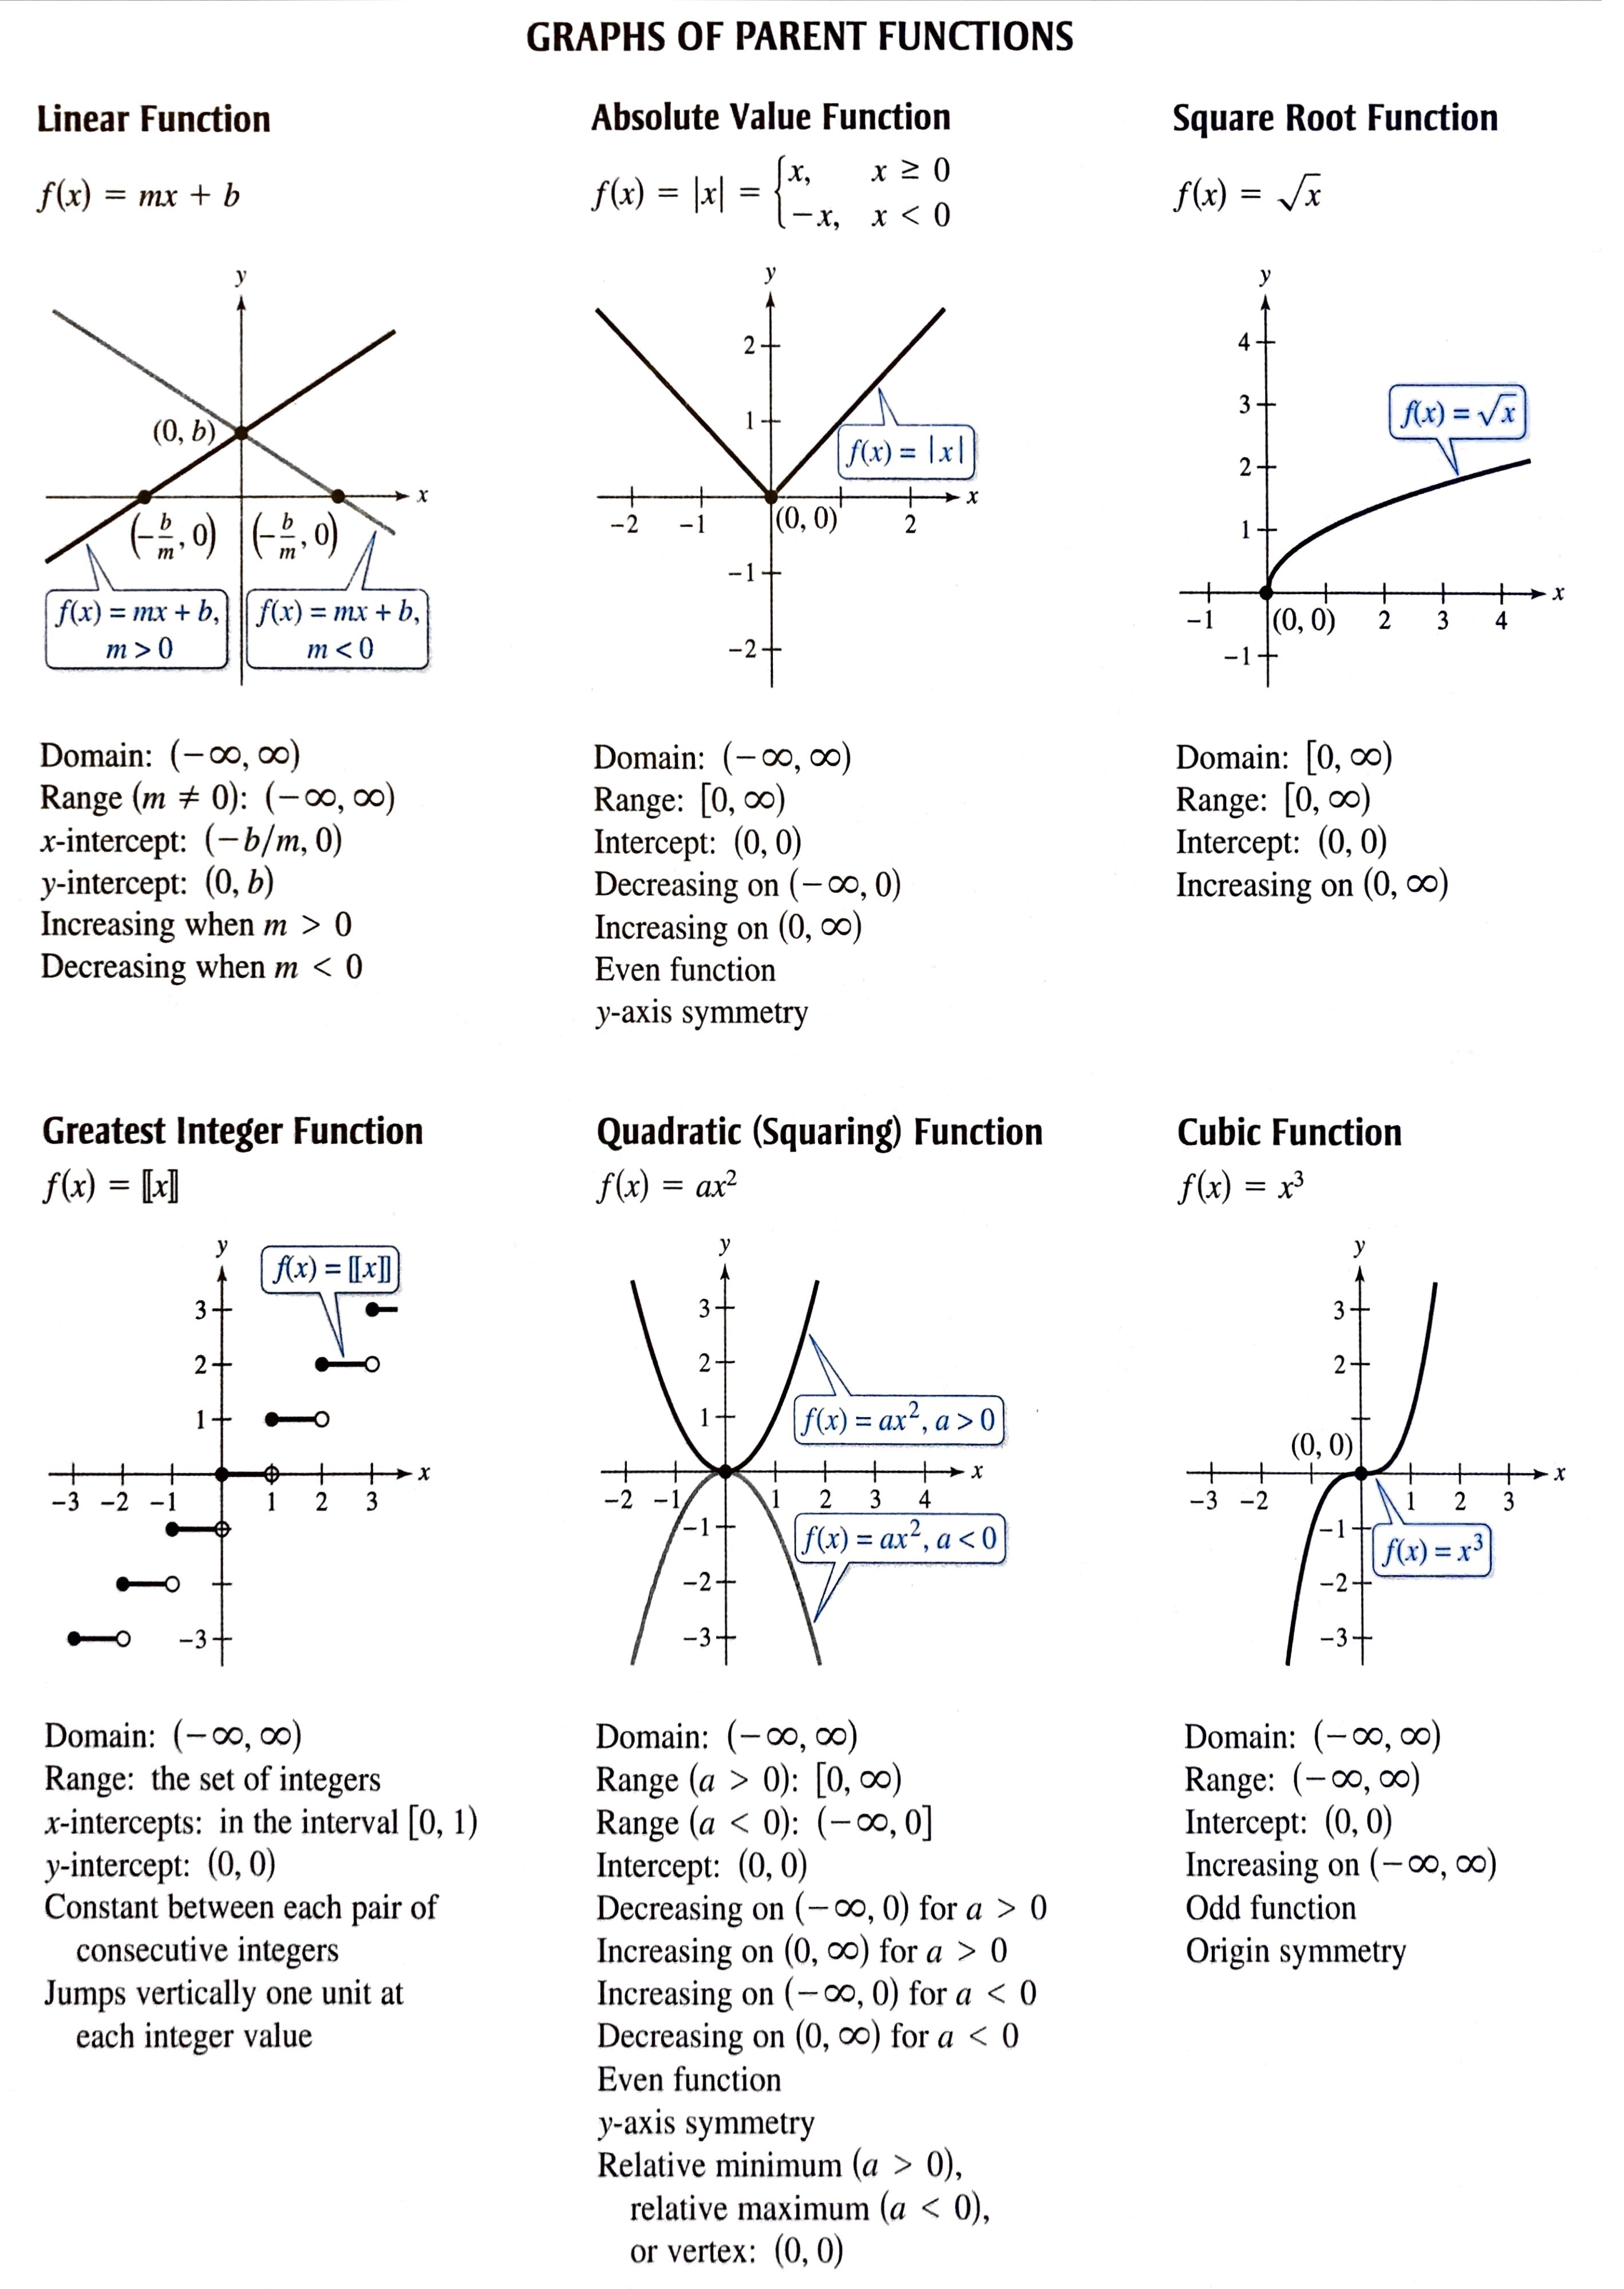
\includegraphics[width=7.6cm]{parent1}
	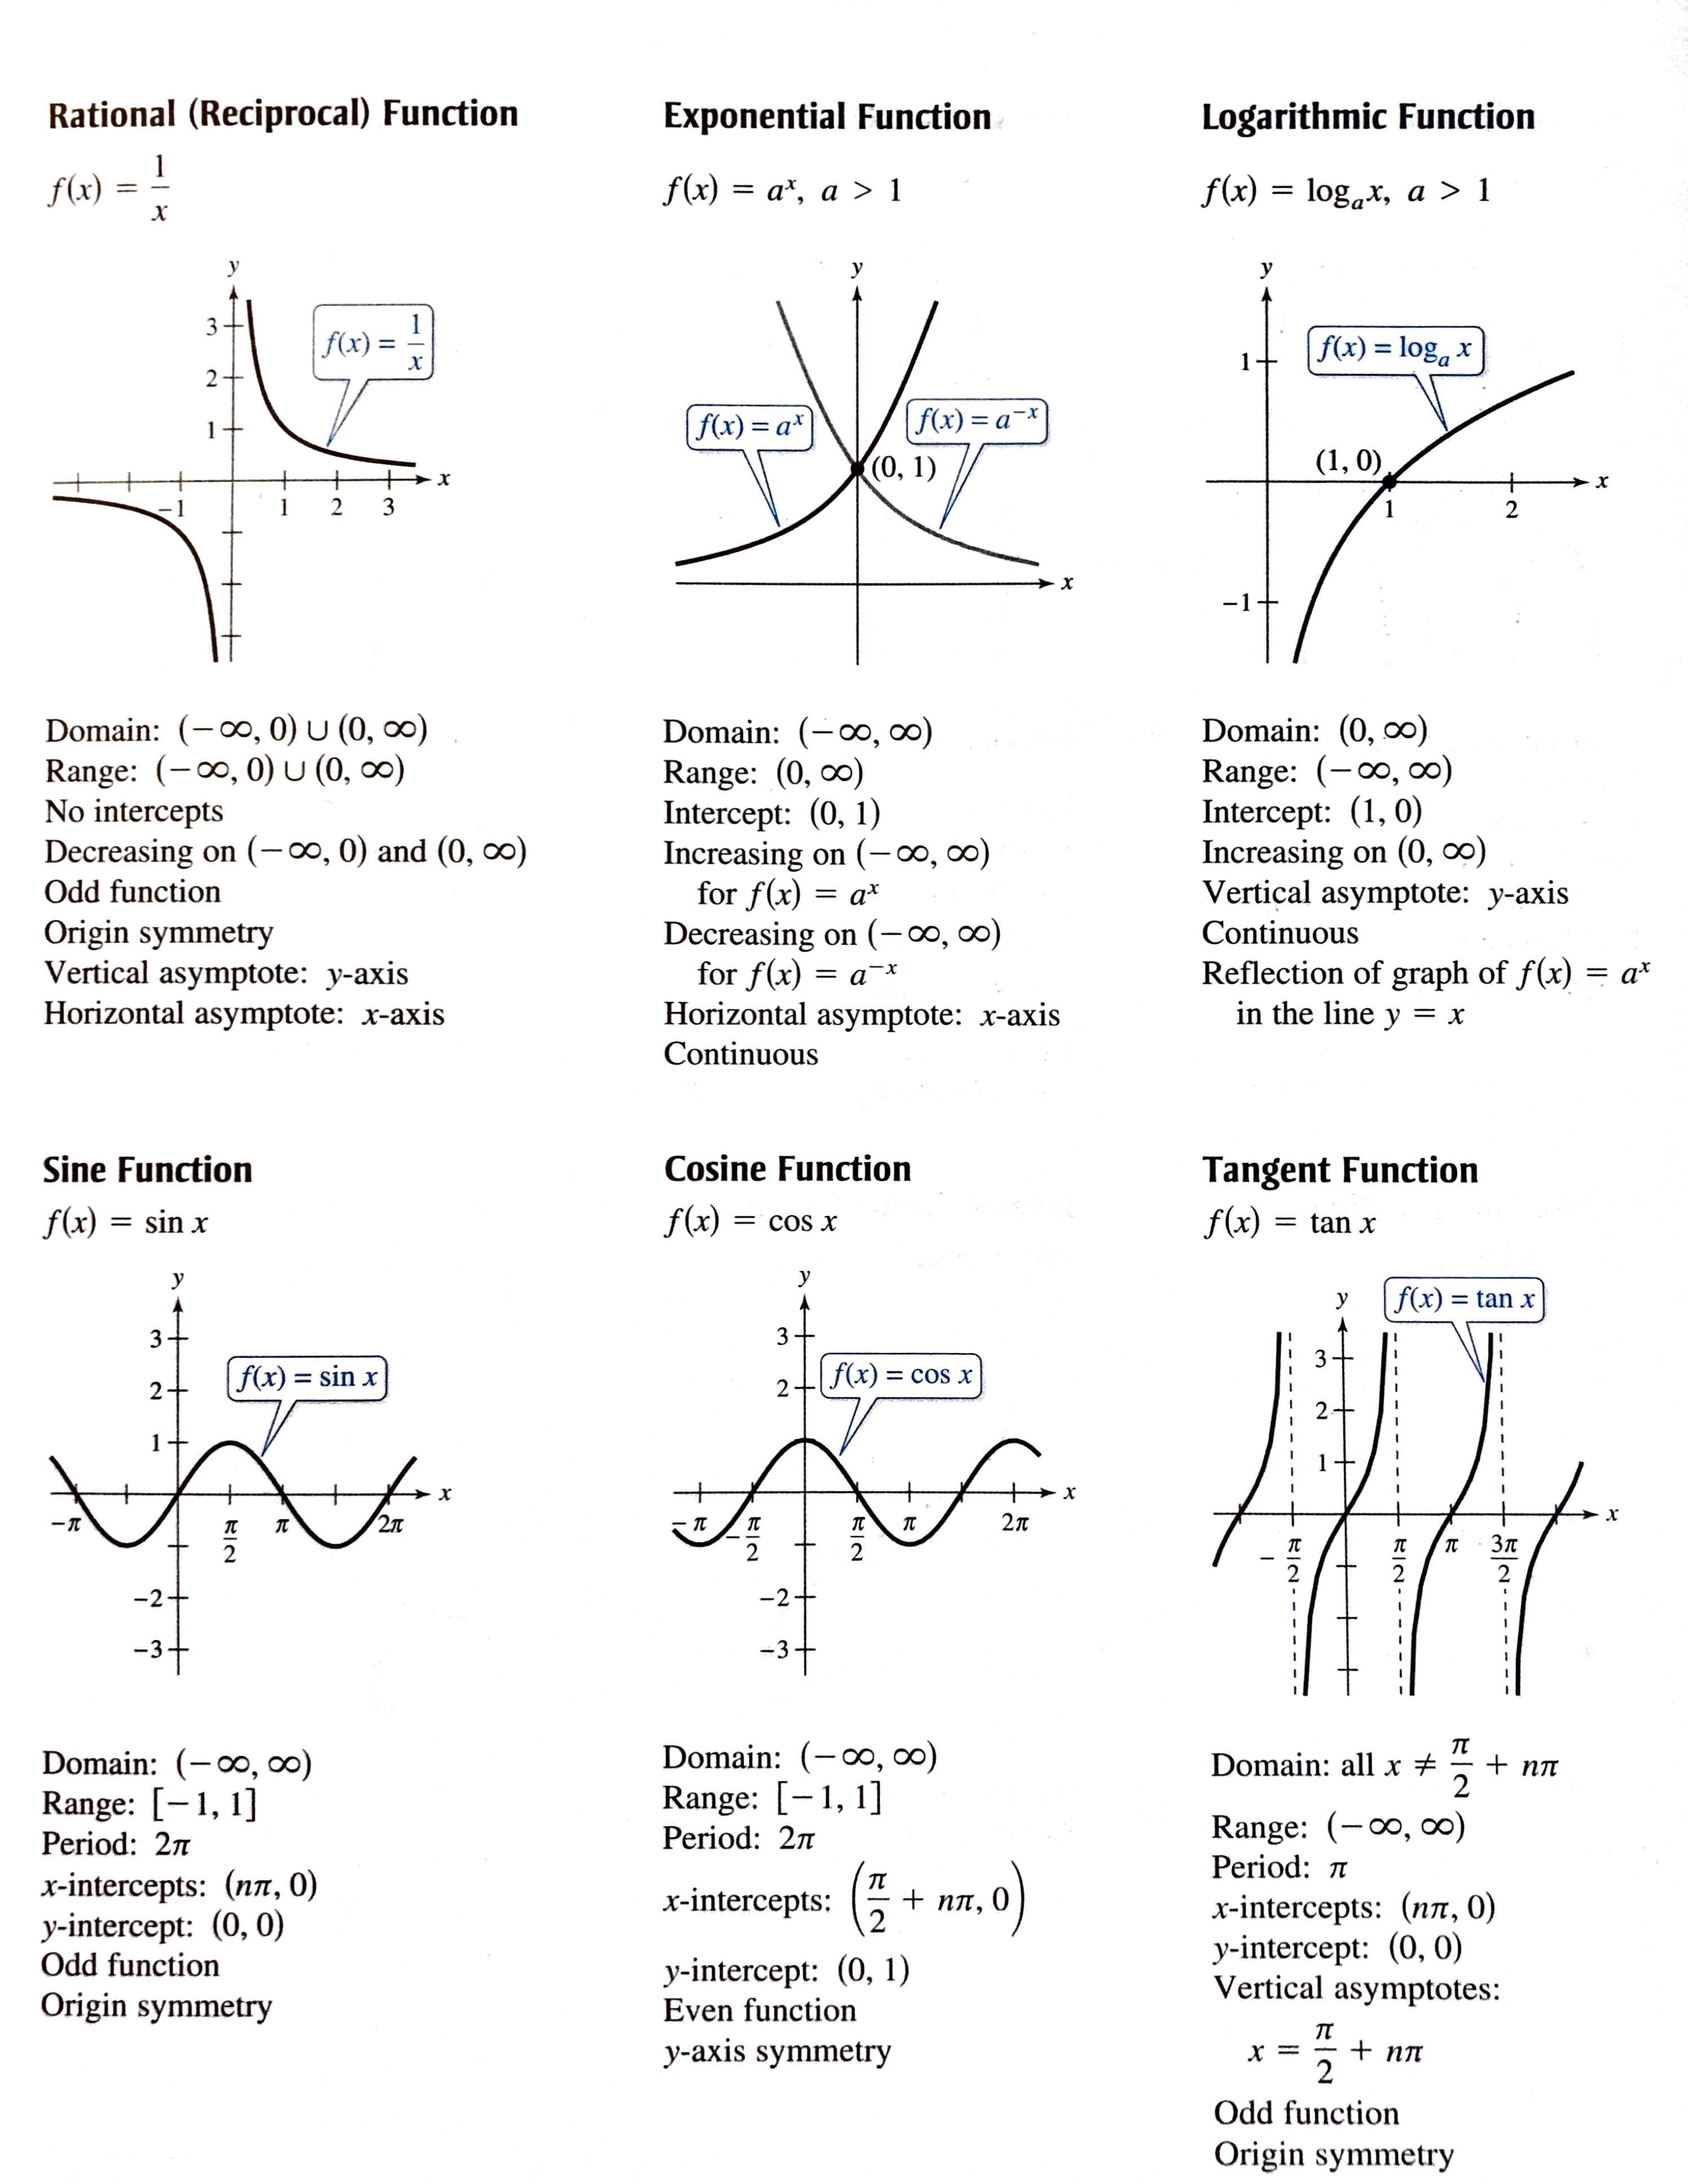
\includegraphics[width=7.6cm]{parent2}
\end{figure}

% \end{figure}
\subsection{Transformations}
Let \(c\) be a positive real number. Vertical and horizontal shifts in the graph of
\(y=f(x)\) are represented as follows.
\begin{enumerate}
	\item Vertical shift \(c\) units \emph{up}: \quad \( h(x) = f(x) + c \)
	\item Vertical shift \(c\) units \emph{down}: \quad \(h(x) =f(x) - c\)
	\item Horizontal shift \(c\) units to the right:\quad \(h(x) =f(x-c)\)
	\item Horizontal shift \(c\) units to the left:\quad  \(h(x) = f(x+c)\)
	\item Reflection on x-axis: \quad \(h(x)=-f(x) \)
	\item Reflection on y-axis: \quad \(h(x)=f(-x),  \)
	\item Vertical Dilation: \quad  \(h(x)=cf(x), |c| > 1 = \mathrm{ stretch}, |c| < 1 = \mathrm{ shrink }\)
	\item Horizontal Dilation: \quad \(h(x)=f(cx), |c| > 1 = \mathrm{ shrink}, |c| < 1 = \mathrm{ stretch }\)
\end{enumerate}

\textbf{Note:} Order matters, therfore note e.g.\ if reflections need to be applied to the entire function after or before other transformations.

\subsection{Inverse Functions}
\begin{enumerate}
	\item Rewrite \(f(x)\) using \emph{y} in place of \emph{x}
	\item Solve for y. The new function is the inverse function \(f^{-1}(x)\) of \(f(x)\)
\end{enumerate}

\subsection{Kinematics \& SUVAT}
The kinematic quantities are:
% Please add the following required packages to your document preamble:
% \usepackage{booktabs}
\begin{table}[H]
	\centering
	\begin{tabular}{@{}ll@{}}
		\toprule
		Variable & Quantity                              \\ \midrule
		s        & displacement                          \\
		u        & initial velocity                      \\
		v        & final velocity                        \\
		a        & acceleration                          \\
		t        & time taken for the change in velocity \\ \bottomrule
	\end{tabular}
\end{table}

The four \emph{SUVAT} equations are:
\begin{align}
v&=u+at \\
v^{2}&=u^{2}+2as 		 \\
s&=u t+\frac{1}{2}at^{2}	\\
s&=v-\frac{1}{2}at^{2}		\\
s&=\frac{1}{2}(u+v)t
\end{align}
\section{Angles \& Triangles}
\subsection{Types of Triangles}
The following lists the common types of triangles.

\begin{figure}[H]
	\centering
	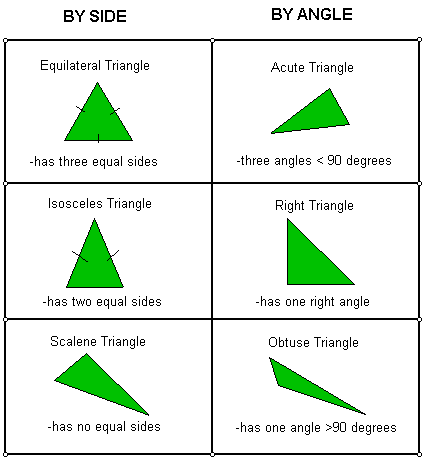
\includegraphics[width=8cm]{triclass}
\end{figure}
\subsection{Triangle Invariants}
\paragraph{Angle Sum}
The sum of all angles  in a triangle is always 180\degree{} or \( \pi \) rad.
\[
	\alpha + \beta + \gamma = 180 \degree = \pi \mathrm{rad}
\]
\paragraph{Triangle Inequality}
The sum of two sides is strictly larger than the third side.

\[
	a + b > c
\]

\subsection{Radians and Degrees}
\begin{mdframed}
\textbf{Calculator Hint:} Use \keystroke{math} \keystroke{DMS} to convert between radians and degrees.
\end{mdframed}

\begin{enumerate}
	\item To convert degrees to radians, multiply degrees by \(\frac{\pi \mathrm{rad}}{180^{\circ}}\)
	\item To convert radians to degrees, multiply radians by \(\frac{180^{\circ}}{\pi \mathrm{rad}}\)
	      \begin{figure}[H]
	      	\centering
	      	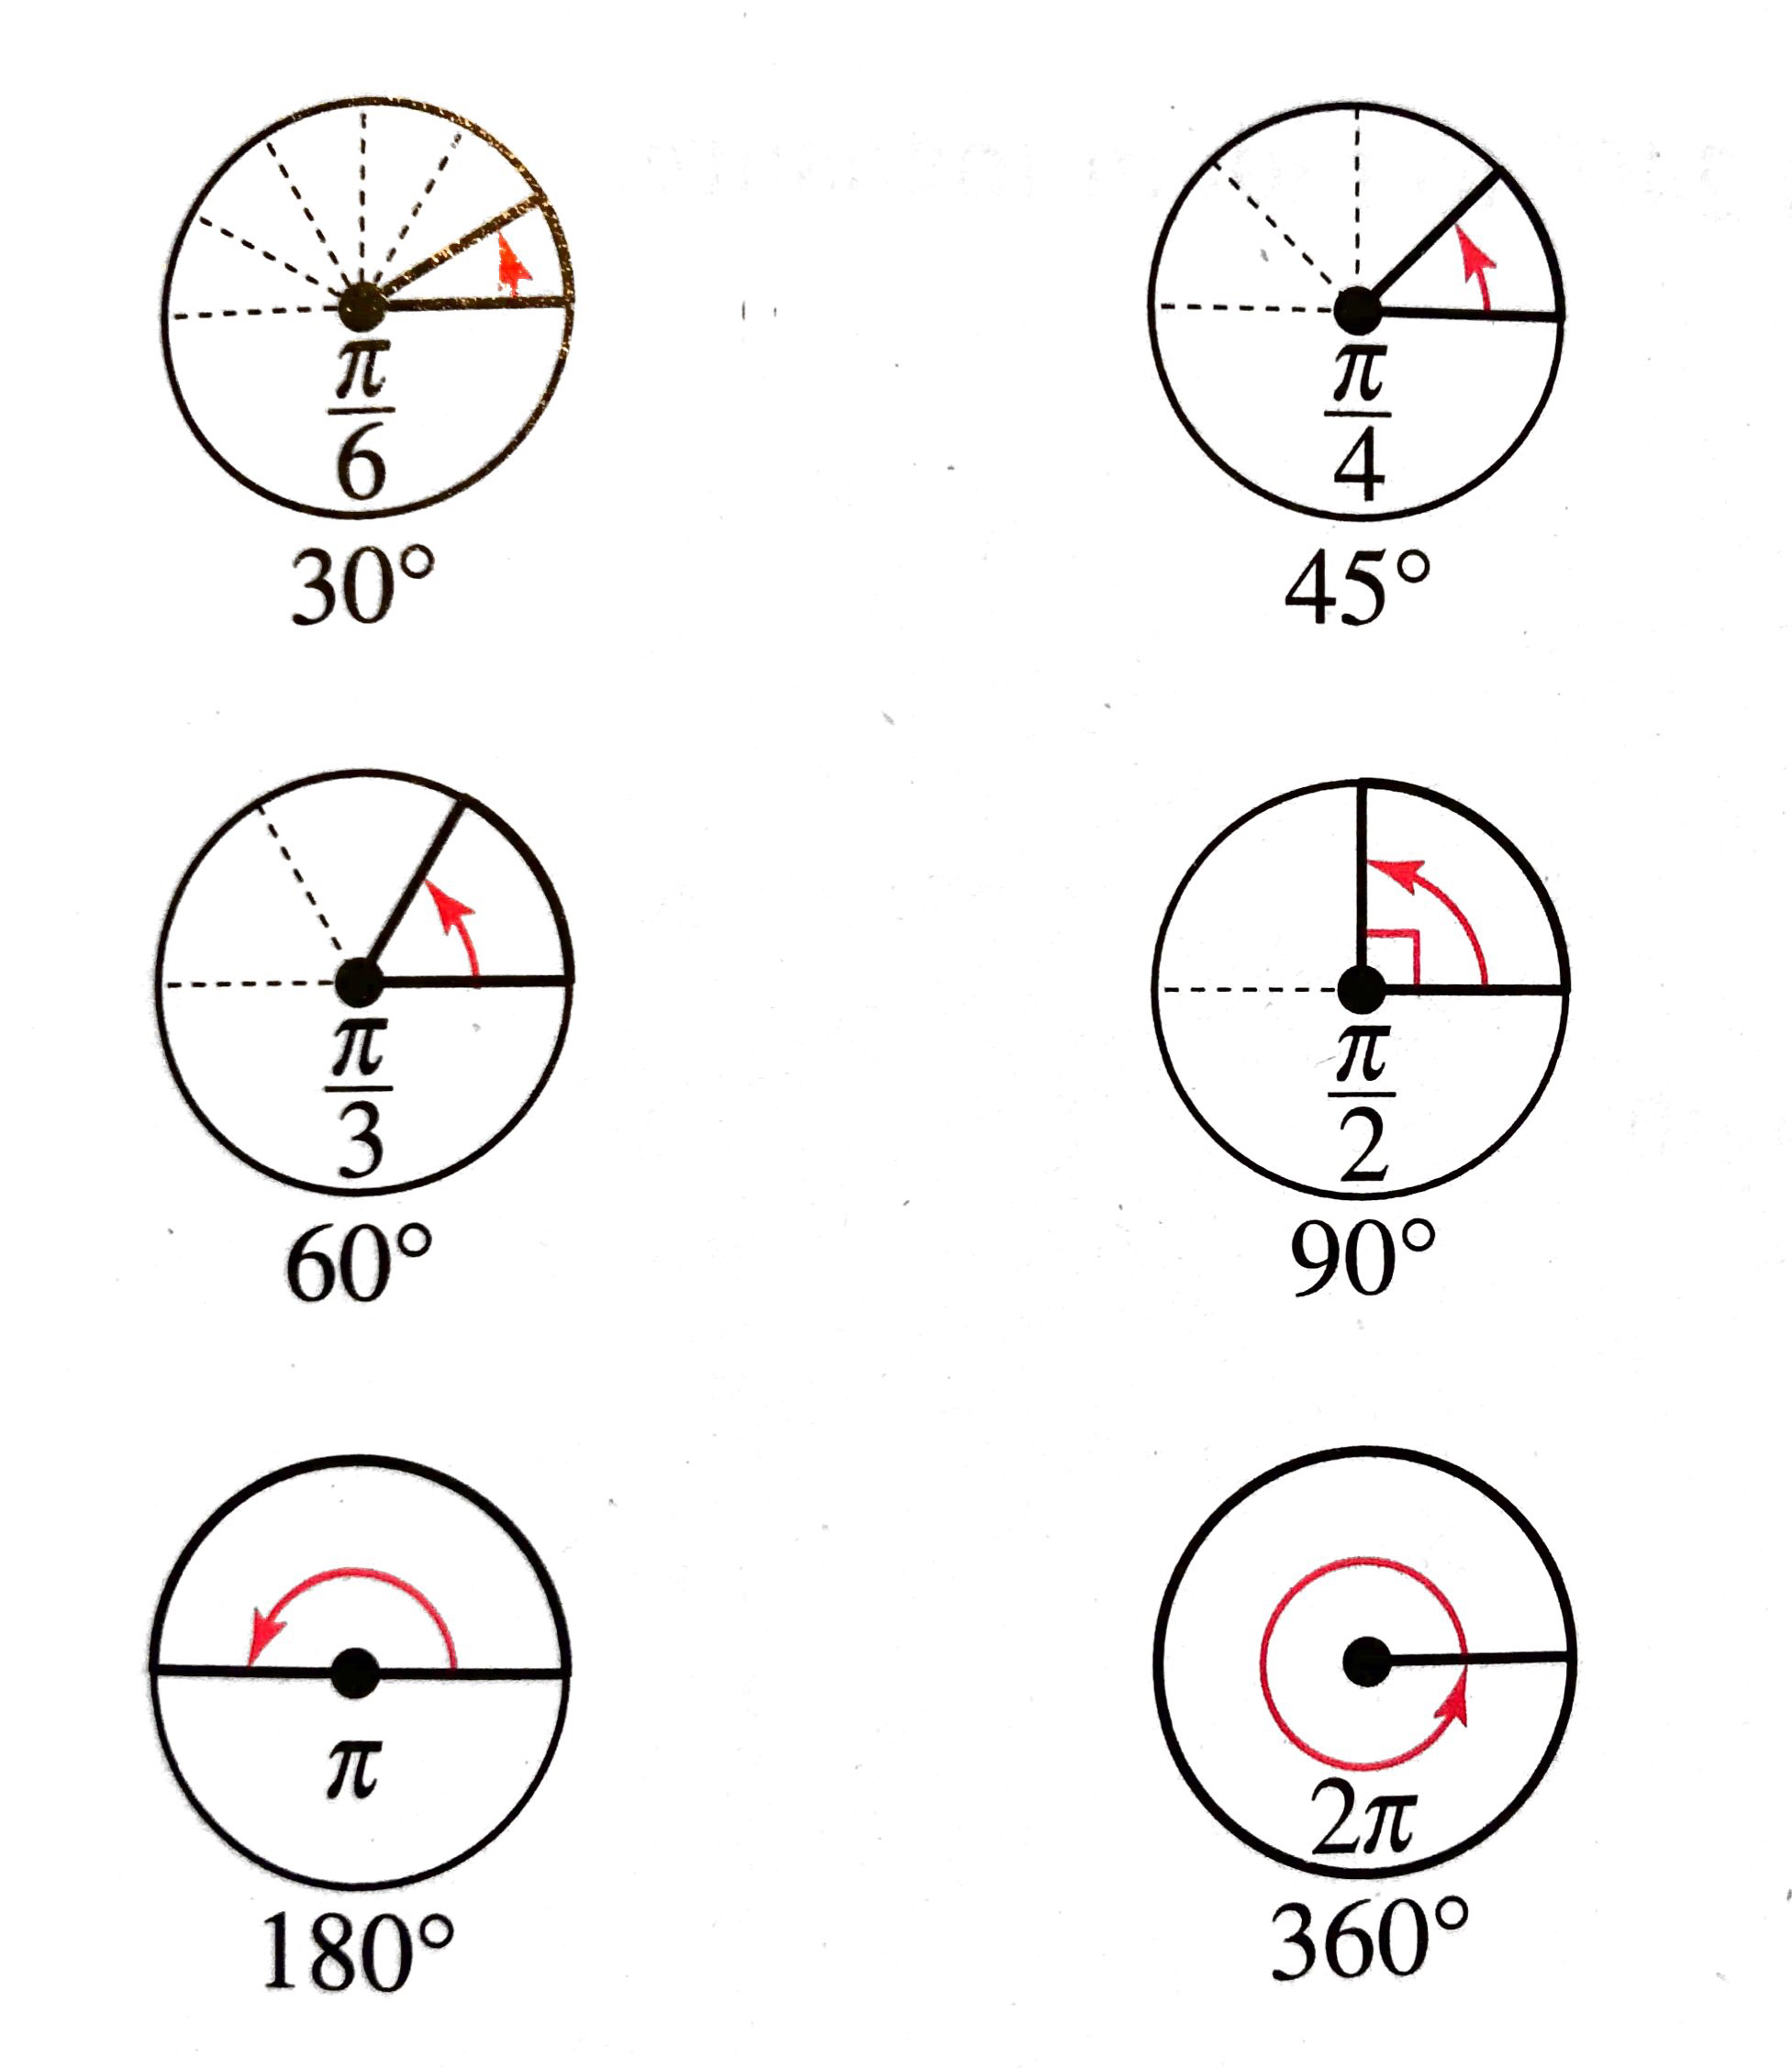
\includegraphics[width=6cm]{rads}
	      \end{figure}
\end{enumerate}

\subsection{Working with Surds}
Working with roots (surds, radicals), these properties should be kept in mind.

\begin{align*}
	\sqrt[n]{a^{m}}                 & ={(\sqrt[n]{a})}^{m}                   \\
	\sqrt[n]{a} \cdot \sqrt[n]{b}   & =\sqrt[n]{a b}                         \\
	\frac{\sqrt[n]{a}}{\sqrt[n]{b}} & =\sqrt[n]{\frac{a}{b}}, \quad b \neq 0 \\
	\sqrt[m]{\sqrt[n]{a}}           & =\sqrt[m n]{a}                         \\
	\sqrt[n]{a}^{n}                 & =a                                     \\
	\sqrt[n]{a^{n}}                 & =|a|, n                                \\
	\sqrt[n]{a^{n}}                 & =a                                     \\
	a^{1 / n}                       & =\sqrt[n]{a}
\end{align*}


\section{Trigonometric Functions}

\subsection{Trigonometric Ratios in Right Triangles}
The main trigonometric rations are as follows.
\begin{align} \sin \theta &=\frac{\mathrm{opp}}{\mathrm{hyp}} \\ \cos \theta &=\frac{\mathrm{adj}}{\mathrm{hyp}} \\ \tan \theta &=\frac{\mathrm{opp}}{\mathrm{adj}} \end{align}
Further, the following identities are important.

\begin{align}
	\sin ^{2} A+\cos ^{2} A & =1                                     \\
	\frac{\sin A}{\cos A}   & =\tan A                                \\
	\sin \theta             & =-\sin \left(\theta-180^{\circ}\right) \\
	\cos \theta             & =-\cos \left(\theta-180^{\circ}\right) \\
	\tan \theta             & =\tan \left(\theta-180^{\circ}\right)  \\
	\sin \theta             & =-\sin \left(360^{\circ}-\theta\right) \\
	\cos \theta             & =\cos \left(360^{\circ}-\theta\right)  \\
	\tan \theta             & =-\tan \left(360^{\circ}-\theta\right) \\
\end{align}

\subsection{Trigonometric Laws}

\subsubsection{Law of Sines}

The sine rule states
\begin{align}
	\frac{a}{\sin A}=\frac{b}{\sin B}=\frac{c}{\sin C}
\end{align}

This rule can \emph{only} be used when given two angles and one side, or two sides and a non-included angle.

\subsubsection{Law of Cosines}

The cosine rule states

\begin{align}
	a^{2} & =b^{2}+c^{2}-2 b c \cos A \\
	b^{2} & =a^{2}+c^{2}-2 a c \cos B \\
	c^{2} & =a^{2}+b^{2}-2 a b \cos C \\
\end{align}

This rule is used when given three sides or two sides and the included angle.
\subsubsection{Application of the Laws}

\begin{table}[ht]
\renewcommand{\arraystretch}{3}
\centering
\begin{tabular}{ccccc}
\toprule
                      Angles / Sides& 1 Side & 2 Sides& 3 Sides \\ \midrule
\multicolumn{1}{c|}{1 Angle} & not solvable & Encl.: Sines, Unencl.: Cosines & Law of Cosines  \\
\multicolumn{1}{c|}{2 Angles} & Law of Sines & Law of Cosines & Law of Cosines &  \\
\multicolumn{1}{c|}{3 Angles} & Law of Sines & Law of Sines & Solved &  \\ \bottomrule
\end{tabular}
\end{table}

When dealing with the case \(SSA\) with enclosed angle, the law of sines can produce two angles as possible answers. In this case:

\begin{enumerate}
	\item See if you are given two sides and the angle not in between (SSA). This is the situation that may have 2 possible answers.
\item  Find the value of the unknown angle.
\item  Once you find the value of your angle, subtract it from 180\degree{} to find the possible second angle.
\item  Add the new angle to the original angle. If their sum is less than 180\degree, you have two valid answers. If the sum is over 180\degree, then the second angle is not valid.
\end{enumerate}


\subsection{Inverses of Trigonometric Functions}
To find an inverse, we need to find a part of the function that is one-to-one. Hence, we restrict the domain of the three trigonmetric functions. Domain and range are flipped.

	      \begin{figure}[H]
	      	\centering
	      	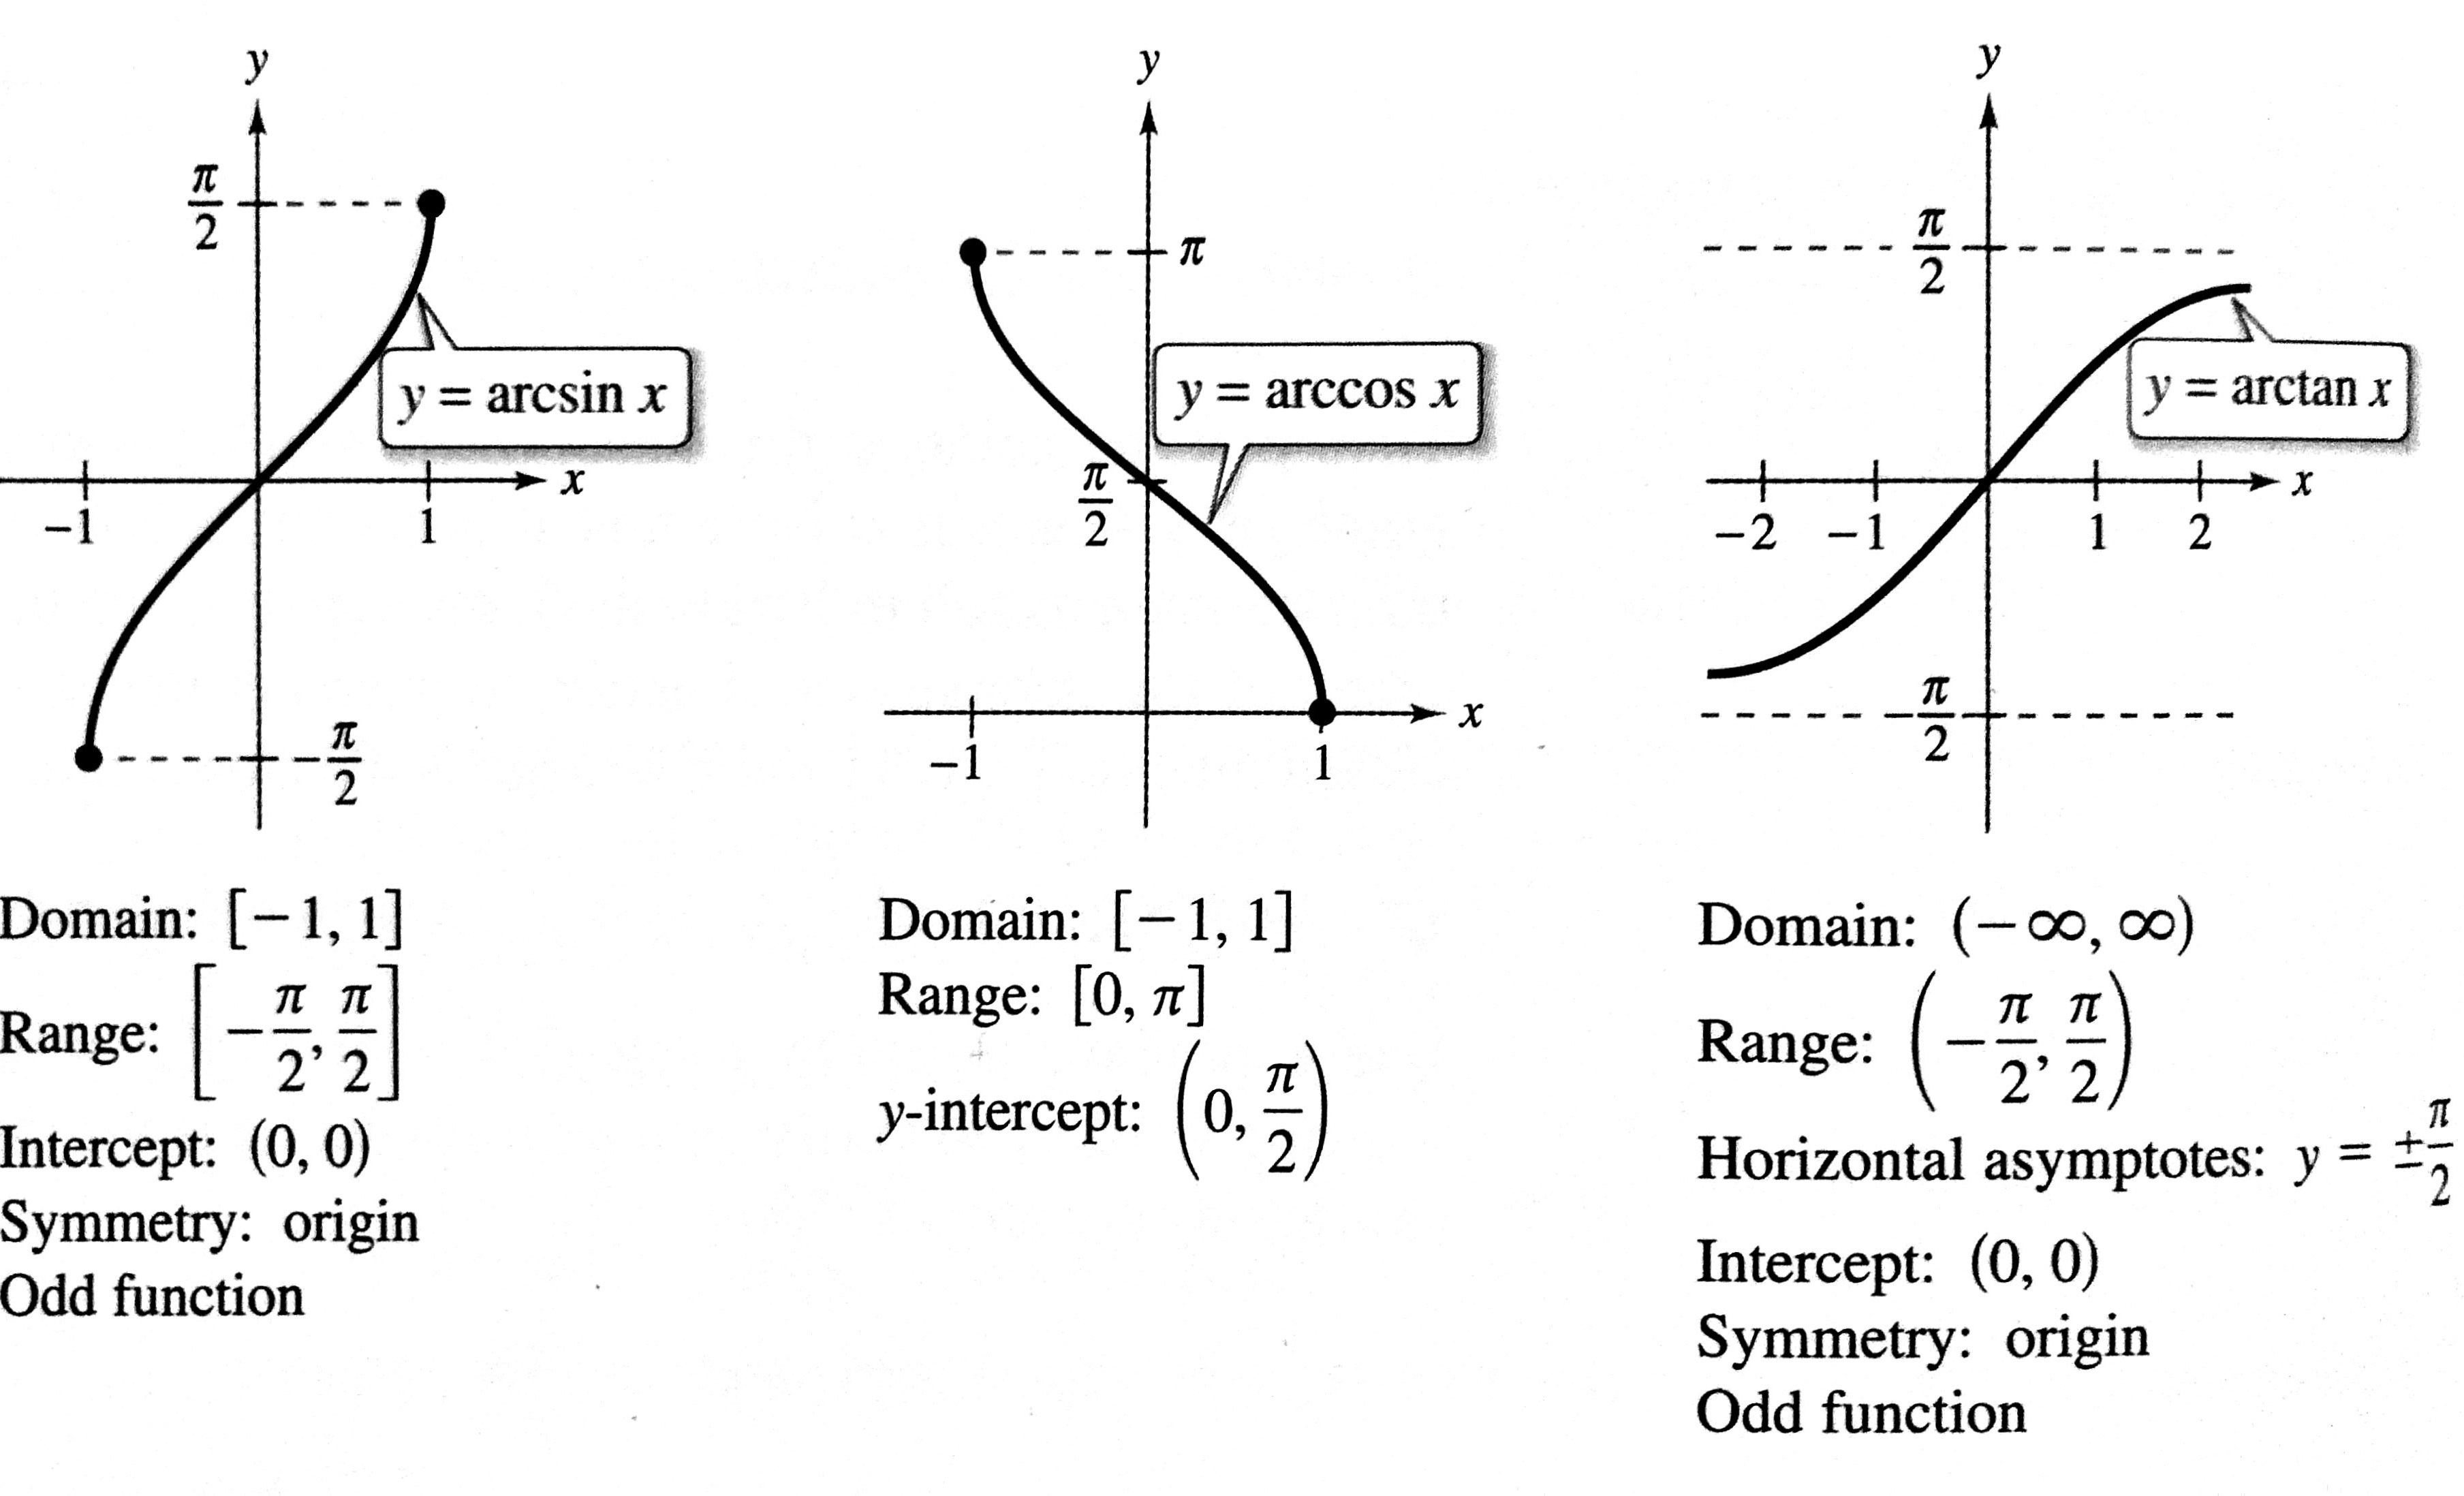
\includegraphics[width=14cm]{triginverse}
	      \end{figure}


\subsection{Transformations of Trigonometric Functions}
Let \(c\) be a positive real number. Vertical and horizontal shifts in the graph of
\(y=f(x)\) are represented as follows.
\begin{enumerate}
	\item Vertical shift \(c\) units \emph{up}: \quad \(h(x)=\sin(x) + c\)
	\item Vertical shift \(c\) units \emph{down}: \quad \(h(x)=\sin(x) - c\)
	\item Horizontal shift \(c\) units to the right:\quad \(h(x)=\sin(x-c)\)
	\item Horizontal shift \(c\) units to the left:\quad  \(h(x)=\sin(x+c)\)
	\item Reflection on x-axis: \quad \(h(x)=-\sin(x)\)
	\item Reflection on y-axis: \quad \(h(x)=\sin(-x)\)
	\item Vertical Dilation, \(c\) is the \emph{amplitude and range}: \quad  \( h(x) = c \sin(x)\)
	\item Horizontal Dilation, \(c\) adjusts the \emph{period}: \quad \(h(x)=f(cx)\)
\end{enumerate}

Remember that \( \sin \) and \( \cos \) are horizontal translations of each other by \(\frac{\pi}{2}\).

\subsection{Solving Trigonometric Equations}

\begin{enumerate}
	\item Check if the question is asking for values of \(x\) within \([0,360\degree]\) or \([-360\degree,360\degree]\)
	\item After solving the equation, ensure covering all possible angles. To do this, find the \emph{corresponding angle} by finding the other angle with the same sign.
	\item For \(\sin(\theta)\), the corresponding angle is \(180\degree - \theta \)
	\item For \(\cos(\theta)\), the corresponding angle is \(360\degree - \theta \)
	\item For \(\tan(\theta)\), the corresponding angle is \(\theta + 180\degree \)
	\item Finally, calculate two further angles by subtracting \( 360k, k = -1 \) from them (if these are in range).
\end{enumerate}

\subsection{Polar Coordinates}

\begin{mdframed}
\textbf{Calculator Hint:} Use \keystroke{math} \keystroke{R P} to convert between polar and cartesian. Note that you can only receive output of one coordinate at a time (\(x,y,r,\theta \)).
\end{mdframed}

\paragraph{Cartesian to Polar}
\begin{align}
	r      & = \sqrt{x^2+y^2}         \\
	\theta & = \tan^{-1}(\frac{y}{x})
\end{align}

\paragraph{Polar to Cartesian}
\begin{align}
	x & = r \cos(\theta) \\
	y & = r \sin(\theta)
\end{align}

\section{Exponential Functions \& Logarithms}

\subsection{Exponential Functions}
\(e\) is the exponential constant 2.71828\ldots Exponential expressions can be simplified using the rules below.

\begin{align}
	\mathrm{e}^{a} \mathrm{e}^{b}         & =\mathrm{e}^{a+b} \\[20pt]
	\frac{\mathrm{e}^{a}}{\mathrm{e}^{b}} & =\mathrm{e}^{a-b} \\[20pt]
	\mathrm{e}^{0}                        & =1                \\[20pt]
	{(e^a)}^{b}                           & =\mathrm{e}^{a b}
\end{align}

The exponential function is

\begin{equation}
	y = e^x
\end{equation}

\begin{itemize}
	\item The exponential function is never negative.
	\item When \(x = 0\), the function value is 1.
	\item As \(x\) increases, then \(e^x\) increases. This is known as \emph{exponential growth}.
\end{itemize}

\subsection{Logarithmic Functions}

\paragraph{Logarithm}
\(y = a^x \)and \(\log_{a} y = x\) are equivalent. The notation \(\log_{5} 125 = 3\) is read as ``The logarithm to the base 5 of 125 is 3.'' The following identities are of importance.

\begin{align}
	\log_a X & = \frac{\log_{10} X}{\log_{10} a} \\[20pt]
	\log_a X & = \frac{\ln X}{\ln a}             \\[20pt]
	\log_a a & = 1                               \\[20pt]
	\log_a 1 & = 0
\end{align}
\subsubsection{Laws of Logarithms}
\paragraph{Product Property} \(\log A + \log B = \log AB\)
\paragraph{Quotient Property} \(\log A - \log B = \log \frac{A}{B}\)
\paragraph{Power Property} \(n \log A  = \log A^n\)

Some useful identities to solve equations are listed below. Note that even if an equation has solutions, these may not be valid given the original equation (e.g.\ negative values in a \(\log \)function). Use the \textbf{inverse} and \textbf{one-to-one} properties to solve these equations.

\begin{align}
	\ln(e^x)   & = x \\
	e^{\ln(x)} & = x
\end{align}

\section{Limits \& Differentiation}

\subsection{Limits}
If \(f(x)\) become arbitrarily close to a unique number \(L\) as \(x\) approaches \(c\) from either side, then the \textbf{limit} of \(f(x)\) as \(x\) approaches \(c\) is \(L\).
\begin{equation}
	\lim_{x \to c}f(x) = L
\end{equation}

\subsubsection{Estimating Limits}
\begin{enumerate}
	\item Check what the variable is supposed to approach
	\item Build a table of values that allows you to investigate the approached x-value
	\item Investigate the limit. It may be that the function is not defined at the approached x-value. The limit may still exist.
	\item Check if the limit can exist (see below).
\end{enumerate}

\subsubsection{Conditions Under Which Limits Do Not Exist}
The limit of \(f(x)\) as \(x \rightarrow c\) does not exist when any of the
conditions listed below are true.
\begin{enumerate}
	\item \(f(x)\) approaches a different number from the right side of \(c\)
	      than it approaches from the left side of \(c\).
	\item \(f(x)\) increases or decreases without bound as \(x\) approaches \(c\).
	\item \(f(x)\) oscillates between two fixed values as \(x\) approaches \(c\).
\end{enumerate}

\subsubsection{Basic Limits}

Let \(b\) and \(c\) be real numbers and let \(n\) be a positive integer. Using the properties below, you can use \textbf{direct substitution} to evaluate the limit.

\[
	\lim_{x \to c} f(x) = f(c)
\]

\begin{align}
	\lim_{x \to c}b           & = b           & \text{Limit of a constant function}   \\
	\lim_{x \to c}x           & = c           & \text{Limit of the identity function} \\
	\lim_{x \to c}x^n         & = c^n         & \text{Limit of a power function}      \\
	\lim_{x \to c}\sqrt[n]{x} & = \sqrt[n]{c} & \text{Limit of a radical function}
\end{align}

\subsubsection{Properties of Limits}
Let \(b\) and \(c\) be real numbers, let \(n\) be a positive integer, and let \(f\) and \(g\) be functions with the limits \(\lim _{x \rightarrow c} f(x)=L\) and \(\lim _{x \rightarrow c} g(x)=K\)

\begin{align}
	\lim_{x \to c} [b f(x)]          & =b L \quad                   \\
	\lim_{x \to c}[f(x) \pm g(x)]    & =L \pm K                     \\
	\lim_{x \to c}[f(x) g(x)]        & =L K \quad                   \\
	\lim_{x \to c} \frac{f(x)}{g(x)} & =\frac{L}{K} \quad, K \neq 0 \\
	\lim_{x \to c}{[f(x)]}^{n}       & =L^{n}
\end{align}

\subsubsection{Dividing out \& Rationalising}
\begin{enumerate}
	\item If direct subsitution fails, e.g.\ it produces a quotient such as \(\frac{0}{0}\), try factorising or rationalising (multiply by the conjugate) the denominator or numerator
	\item Divide out any common factors
	\item Use direct substitution on the newly formed function
\end{enumerate}

\subsubsection{Limits at Infinity}

If \(r\) is a real positive number, then
\[
	\lim_{x\to\infty}\frac{1}{x^r} = 0
\]


Given a function in rational form \(\frac{f(x)}{g(x)}\), if the order of both numerator and denominator are the same, the limit is composed of the leading coefficients of the highest order.


Otherwise, use the following technique:
\begin{enumerate}
	\item Divide both numerator and denominator by the highest power in the denominator
	\item Evaluate the limits of individual terms; fractions with \(x\) in the denominator evaluate to 0.
\end{enumerate}

\subsection{Differentiation}

A gradient function \( f'(x) \)describes the slope of the tangent line at any point of a function \(f(x)\). It is also called the \textbf{first derivative}.

\subsubsection{Common Functions}
\autoref{tab:derivatives} lists common functions and their first derivatives.
% Please add the following required packages to your document preamble:
% \usepackage{booktabs}
\begin{table}[ht]
	\caption{Common functions \& their derivatives}\label{tab:derivatives}
\centering
	\renewcommand{\arraystretch}{2}
	\setlength{\tabcolsep}{12pt}
	\begin{tabular}{@{}lll@{}}

		\toprule
		Function     & \(f(x)\)        & \(f'(x)\)                         \\ \midrule
		Constant     & \(c\)               & 0                                 \\
		Line         & \(x\)               & 1                                 \\
		Square       & \(x^2\)         & \(2x\)                            \\
		Square Root  & \(\sqrt{x}\)    & \(\frac{1}{2}x^{-\frac{1}{2}}\)   \\
		Exponential  & \(e^x\)         & \(e^x\)                           \\
		             & \(a^x\)         & \(\ln(a)a^x\)                     \\
		Logarithms   & \(\ln(x)\)      & \(\frac{1}{x}\)                   \\
		             & \( \log_a(x) \) & \( \frac{1}{\ln(a)x} \)            \\
		Trigonometry & \(\sin(x) \)    & \(\cos(x)  \)                     \\
		             & \( \cos(x) \)   & \(-\sin(x) \)                     \\
		             & \( \tan(x) \)   & \( \frac{1}{\cos^2(x)} = \sec^2\) \\ \bottomrule
	\end{tabular}

\end{table}

\subsubsection{Differentiation Rules} % (fold) \label{ssub:subsubsection_name}
\autoref{tab:diffrules} lists the most important rules to find the derivative of a function.
\begin{table}[ht]
	\caption{Differentiation Rules}\label{tab:diffrules}
	\centering
	\renewcommand{\arraystretch}{2}
	\begin{tabular}{m{0.2\textwidth}m{0.4\textwidth}m{0.3\textwidth}}
		\toprule


		Rule                         & \(f(x)\)        & \(f'(x)\)                 \\ \midrule
		Multiplication by a constant & \(cf\)          & \(cf'(x)\)                \\
		Power Rule                   & \( x^n \)       & \(nx^{n-1}\)              \\
		Sum Rule                     & \(f + g\)       & \( f' + g'\)              \\
		Difference Rule              & \(f - g\)       & \( f' - g'\)              \\
		Product Rule                 & \(fg\)          & \(f'g + fg'\)             \\
		Quotient Rule                & \(\frac{f}{g}\) & \(\frac{f'g - fg'}{g^2}\) \\
		Reciprocal Rule              & \(\frac{1}{f}\) & \(-\frac{f'}{f^2}\)       \\
		Chain Rule                   & \(f(g(x))\)     & \(f'(g(x))g'(x)\)         \\ \bottomrule
	\end{tabular}

\end{table}

\subsubsection{Finding Minima \& Maxima}
Stationary points are found by setting the gradient function to 0, i.e.\  \(f' = 0\).

Using the second derivative \(f''(x)\), the point can be tested further:

\begin{enumerate}
	\item If \(f''\) is \textbf{positive} at a stationary point, then the point is a \textbf{minimum}.
	\item If \(f''\) is \textbf{negative} at a stationary point, then the point is a \textbf{maximum}.
	\item If \(f''\) is 0, this test does not tell us anything and the points to the left and right of \( f'(x) \) should be examined. This might indicate a point of inflection.
\end{enumerate}

\subsubsection{Finding Asymptotes} % (fold)

\paragraph{Vertical Asymptotes} These are found by finding points where a function \(f(x)\) is undefined. In rational functions, these can be found by finding points where the denominator is 0.

\paragraph{Horizontal Asymptotes} These are found by finding the limit of a function \(f(x)\) as \(x\) approaches \( \infty \). A function can at most have two horizontal asymptotes, one in each direction.

\section{Vectors \& Matrices}

\subsection{Vectors} % (fold)

A vector has both magnitude and direction. A \textbf{unit vector} has magnitude 1. When a vector is multplied by a scalar, it's magnitude is manipulated and the direction remains.

The unit vector \(\hat{a}\) in direction of \(\vec{a}\):

\begin{equation}
	\hat{a} = \frac{1}{|a|}\vec{a}
\end{equation}

The magnitude of a vector:

\begin{equation}
	|\mathbf{a}| = \sqrt{x^2 + y^2}
\end{equation}

\subsubsection{Dot Product}
The dot product of two vectors is a scalar quantity and represents the length of the projection of one vector onto another.

Given two vectors
\[
	\vec{a} =
	\begin{bmatrix}
		a_1 \\ a_2 \\ a_3
	\end{bmatrix}
	, \vec{b} =
	\begin{bmatrix}
		b_1 \\ b_2 \\ b_3
	\end{bmatrix}
\]
the dot product is defined as follows.

\begin{align}
	\vec{a} \bullet \vec{b} & = |a||b|\cos( \theta )     & \text{Geometric Definition} \\
	\vec{a} \bullet \vec{b} & = a_1b_1 + a_2b_2 + a_3b_3 & \text{Algebraic Definition}
\end{align}
\subsubsection{Cross Product}

The cross product of a vector only exists for 2 vectors in a 3-dimensional space. Therefore it can be derived using the Laplace expansion for the \(3 \times 3\) determinant. So, given two vectors \(\vec{a} \times \vec{b}\), we can note a matrix such as

\begin{equation}
	\begin{bmatrix}
		i   & j   & k   \\
		a_1 & a_2 & a_3 \\
		b_1 & b_2 & b_3 \\
	\end{bmatrix}
\end{equation}

Then the cross product's resultant can be calculated using the minor determinants as follows.

\begin{equation}
	\vec{a} \times \vec{b} =
	\begin{vmatrix}
		{v_{2}} & {v_{3}} \\
		{w_{2}} & {w_{3}}
	\end{vmatrix}
	i -
	\begin{vmatrix}
		{v_{1}} & {v_{3}} \\
		{w_{1}} & {w_{3}}
	\end{vmatrix}
	j+
	\begin{vmatrix}
		{v_{1}} & {v_{2}} \\
		{w_{1}} & {w_{2}}
	\end{vmatrix}
	k
\end{equation}

This is a similar approach as the \textbf{Laplace expansion}.

A geometric definition of the \textbf{magnitude} of the cross product is given as

\begin{equation}
	\|\vec{a} \times \vec{b}\|=\|\mathbf{a}\| \|\mathbf{b}\| \sin \theta
\end{equation}

\subsection{Matrices}
\subsubsection{Systems of Linear Equations}
A system of linear equations

\begin{equation}
	\text { System: }\left \{\begin{array}{r}{x-4 y+3 z=5} \\ {-x+3 y-z=-3} \\ {2 x-4 z=6}\end{array}\right.
\end{equation}

can be written as an augmented matrix

\begin{equation}
	\begin{array}{l}{\text { Augmented: }\left[\begin{array}{rrrrr}{1} & {-4} & {3} & {\vdots} & {5} \\ {-1} & {3} & {-1} & {\vdots} & {-3} \\ {2} & {0} & {-4} & {\vdots} & {6}\end{array}\right]}\end{array}
\end{equation}

This form can be used to solve the system by applying elementary row operations to achieve a \textbf{row-echelon form}, which means the matrix has a 1 along the diagonal and zeroes in all positions below the diagonal.

\subsubsection{Elementary Row Operations}
The elementary row operations are:

\begin{equation}
	\begin{array}{ll}{\text { Interchange two rows. }} & {R_{a} \leftrightarrow R_{b}} \\ {\text { Multiply a row by a nonzero constant. }} & {c R_{a} \quad(c \neq 0)} \\ {\text { Add a multiple of a row to another row. }} & {c R_{a}+R_{b}}\end{array}
\end{equation}

\subsubsection{Matrix Addition \& Scalar Multiplication}
Two matrices of the same dimension \(m \times n\) can be added by adding the individual components of the matrix.

\begin{equation}
	A + B = [a_{ij} + b_{ij}]
\end{equation}

A matrix can be multiplied with a scalar by multiplying each component with the scalar.

\begin{equation}
	cA = [ca_{ij}]
\end{equation}

\subsubsection{Matrix Multiplication}

Two matrices can multiplied if and only if the columns of the first matrix matches the number of rows of the second matrix. A matrix with dimensions \(m \times n \) multiplied with a matrix of dimensions \(n \times q\) will result in a matrix of dimensions \(m \times q\).

To calculate the component \(c_{ij}\) of a matrix \(AB\), multiply each \(i\)th row-component of \(A\) with the \(j\)th column-component of \(B\) and add them together.

\subsubsection{Identity Matrix}

The identity matrix \(\mathbf{I} \) is the matrix with leading ones across the diagonal and zeroes everywhere else. It is always \textbf{square}.

\subsubsection{Determinant of a \texorpdfstring{\( 2 \times 2 \)}{2 by 2} matrix}

The determinant of a \(2 \times 2\) matrix is calculated as follows
\[
	\begin{vmatrix}
		a & b \\
		c & d
	\end{vmatrix}
	=
	ad - bc
\]

\subsubsection{Determinant of a \texorpdfstring{\( m \times n \)}{2 by 2} matrix}
The determinant of a 3 \(\times \)3 matrix can be calculated using Sarrus' rule:
\begin{figure}[H]
	\centering
	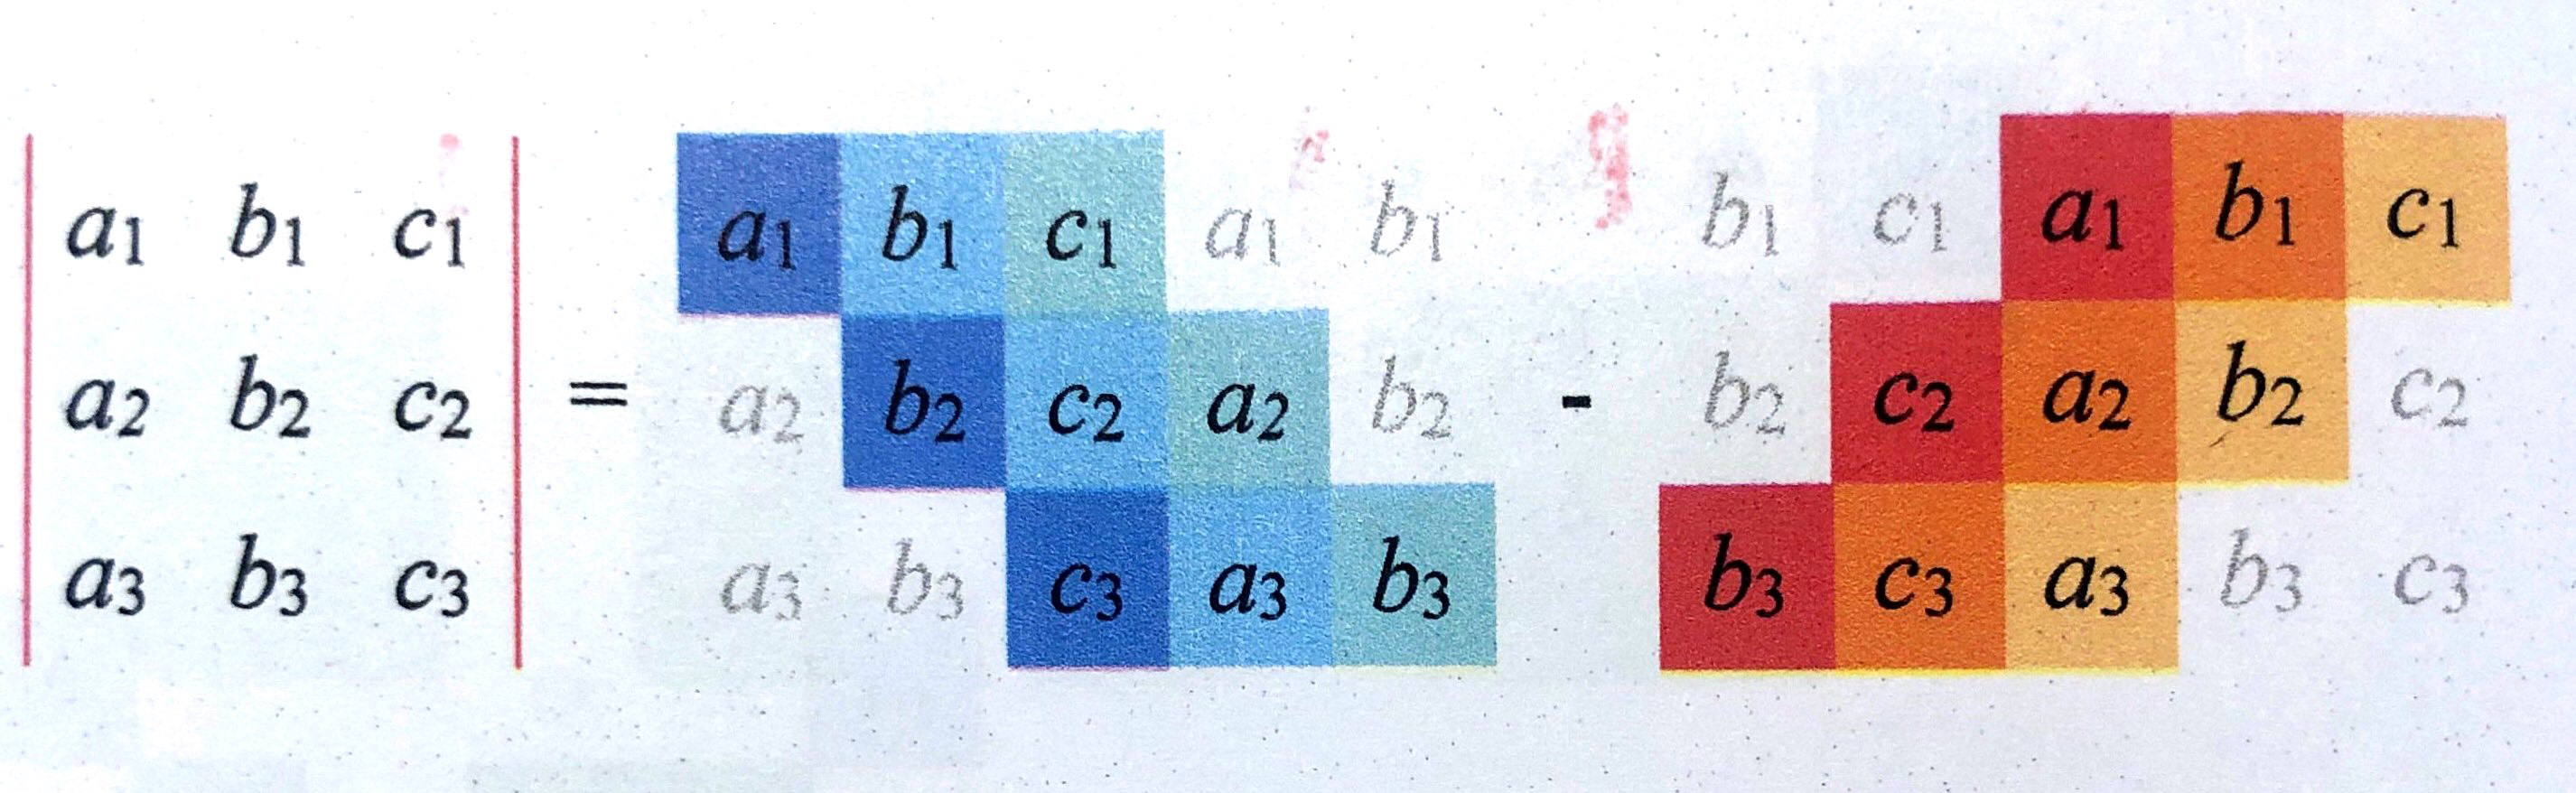
\includegraphics[width=15cm]{Sarrus}
\end{figure}

\begin{equation}
	\det(C) =a_{1} b_{2} c_{3}+b_{1} c_{2} a_{3}+c_{1} a_{2} b_{3}-a_{1} c_{2} b_{3}-b_{1} a_{2} c_{3}-c_{1} b_{2} a_{3}
\end{equation}

For a higher-order matrix, the determinant can be calculated using the \textbf{Laplace expansion}. This multiplies the minor determinants with the elements of the first row and adds them together.

\begin{equation}
		\begin{vmatrix}
			{a_{11} a_{12} a_{13}} \\ {a_{21} a_{22} a_{23}} \\ {a_{31} a_{32} a_{33}}
		\end{vmatrix}
		=a_{11}
		\begin{vmatrix}
			{a_{22} a_{23}} \\ {a_{32} a_{33}}
		\end{vmatrix}
		- 	a_{12}
		\begin{vmatrix}
			{a_{21}} & {a_{23}} \\ {a_{31}} & {a_{33}}
		\end{vmatrix}
		+ a_{13}
		\begin{vmatrix}
			{a_{21}} & {a_{22}} \\ {a_{31}} & {a_{32}}
		\end{vmatrix}
\end{equation}


\subsubsection{Inverse of a \texorpdfstring{\( 2 \times 2 \)}{2 by 2} matrix}
The inverse \( \mathbf{A} \) of a matrix has the property
\begin{equation}
	\mathbf{AA^{-1}} = \mathbf{I}
\end{equation}

The inverse of a \(2 \times 2\) matrix is given by

\begin{equation}
	\mathbf{A}^{-1}=\frac{1}{\det \mathbf{A}}\left[\begin{array}{rr}{d} & {-b} \\ {-c} & {a}\end{array}\right]
\end{equation}

\subsubsection{Inverse of a \texorpdfstring{\( m \times n \)}{2 by 2} matrix}
The inverse of a \(m\times n\) matrix is calculated by building a matrix of cofactors first. This matrix is derived by calculating the \textbf{minor determinants} of the original matrix.

The signs of the cofactor matrix are then flipped to match the following pattern

\begin{equation}
	\left[\begin{array}{l}{+-+} \\ {-+-} \\ {+-+}\end{array}\right]
\end{equation}

The inverse is then given by

\begin{equation}
	A^{-1}=\frac{{(\text { cofactor matrix of } \mathbf{A})}^{\mathrm{T}}}{\text { det } \mathbf{A}}
\end{equation}

\subsection{Transformations}
Transformations on a vector can be expressed as a matrix using homogenous coordinates. These are only needed in the case of translations, otherwise a reduced \(2 \times 2\) transformation matrix may be used.

\paragraph{Translation}

\begin{equation}
	\left[\begin{array}{l}{x^{\prime}} \\ {y^{\prime}} \\ {1}\end{array}\right]=\left[\begin{array}{lll}{1} & {0} & {t_{x}} \\ {0} & {1} & {t_{y}} \\ {0} & {0} & {1}\end{array}\right]\left[\begin{array}{l}{x} \\ {y} \\ {1}\end{array}\right]
\end{equation}

\paragraph{Scaling}

\begin{equation}
	\left[\begin{array}{l}{x^{\prime}} \\ {y^{\prime}} \\ {1}\end{array}\right]=\left[\begin{array}{lll}{s_{x}} & {0} & {0} \\ {0} & {s_{y}} & {0} \\ {0} & {0} & {1}\end{array}\right]\left[\begin{array}{l}{x} \\ {y} \\ {1}\end{array}\right]
\end{equation}


\paragraph{Reflection}
Reflection along the y-axis is given as
\begin{equation}
	\left[\begin{array}{l}{x^{\prime}} \\ {y^{\prime}} \\ {1}\end{array}\right]=\left[\begin{array}{rll}{-1} & {0} & {0} \\ {0} & {1} & {0} \\ {0} & {0} & {1}\end{array}\right]\left[\begin{array}{l}{x} \\ {y} \\ {1}\end{array}\right]
\end{equation}

while reflection along the x-axis is given as

\begin{equation}
	\left[\begin{array}{l}{x^{\prime}} \\ {y^{\prime}} \\ {1}\end{array}\right]=\left[\begin{array}{rrr}{1} & {0} & {0} \\ {0} & {-1} & {0} \\ {0} & {0} & {1}\end{array}\right]\left[\begin{array}{l}{x} \\ {y} \\ {1}\end{array}\right]
\end{equation}

\paragraph{Rotation}
\begin{equation}
	\left[\begin{array}{l}{x^{\prime}} \\ {y^{\prime}} \\ {1}\end{array}\right]=\left[\begin{array}{ccc}{\cos \beta} & {-\sin \beta} & {0} \\ {\sin \beta} & {\cos \beta} & {0} \\ {0} & {0} & {1}\end{array}\right]\left[\begin{array}{l}{x} \\ {y} \\ {1}\end{array}\right]
\end{equation}


\section{Combinatorics \& Probability}
\subsection{Counting Problems}
\subsubsection{Fundamental Counting Principle}

Let \(E_{1}\) and \(E_{2}\) be two events. The first event \(E_{1}\) can occur in \(m_{1}\) different ways:
After \(E_{1}\) has occurred, \(E_{2}\) can occur in \(m_{2}\) different ways. The number of ways
the two events can occur is \(m_{1} \cdot m_{2}\).

\subsubsection{Permutations}
A permutation of \(n\) different elements is an ordering of the elements such tha
one element is first, one is second, one is third, and so on.

\begin{mdframed}
\textbf{Calculator Hint:} Use \keystroke{nPr} to calculate permutations taken \(r\) at a time.
\end{mdframed}

The number of permutations of \(n\) elements is
\[
	\begin{array}{l}{n \cdot(n-1) \cdot \cdot 4 \cdot 3 \cdot 2 \cdot 1=n !} \\ \end{array}
\]
In other words, there are \( n! \) different ways of ordering \(n\) elements.


The number of permutations of \(n\) elements taken \(r\) at a time is

\[
	\nPr{n}{r}=\frac{n !}{(n-r) !}=n(n-1)(n-2) \cdots(n-r+1)
\]

Consider a set of \(n\) objects that has \(n_1\) of one kind of object, \(n_2\) of a second kind, and so on. The number of \textbf{distinguishable permutations} of the \(n\) objects is

\begin{equation}
	\frac{n !}{n_{1} ! \cdot n_{2} ! \cdot n_{3} ! \cdot \cdot \cdot \cdot \cdot n_{k} !}
\end{equation}

\subsubsection{Combinations}

Combinations consider only the possible sets of objects \emph{regardless} of the order in which the members of the set are arranged.

\begin{mdframed}
\textbf{Calculator Hint:} Use \keystroke{nCr} to calculate combinations taken \(r\) at a time.
\end{mdframed}

The number of possible combinations of \(n\) elements taken \(r\) at a time is

\begin{equation}
	\nCr{n}{r}=\frac{n !}{(n-r) ! r !} = \frac{\nPr{n}{r}}{r!}
\end{equation}

\subsection{Probability}
For an event \(E\) with \(n(E)\) outcomes that meet the restriction and that are equally likely, the probability \(P(E)\) of an event within a sample space \(S\) is given as

\begin{equation}
	P(E)=\frac{n(E)}{n(S)}
\end{equation}

The sum of all probabilities of an event must equal 1.

\paragraph{Addition Rule} The probability of two events A \textbf{or} B ocurring is given by

\begin{equation}
	P(A \cup B)=P(A)+P(B)-P(A \cap B)
\end{equation}

If the events are mutually exclusive, then \( P(A \cap B) = 0\)

\paragraph{Multiplication Rule}
The probability of two events A \textbf{and} B ocurring is given by
\begin{equation}
	P(A \cap B)=P(A) \cdot P(B)
\end{equation}

This applies when A and B are independent from each other.

\paragraph{Conditional Probability} The probability of event A ocurring given event B has already ocurred is given by

\begin{equation}
	P(A|B) = \frac{P(A \cap B)}{P(B)}
\end{equation}

The multiplication rule given that A is conditional to B is given by

\begin{equation}
	P(A \cap B) = P(A) \cdot P(B|A)
\end{equation}

\subsection{Statistics}
\subsubsection{Mean}

\paragraph{Mean of a Population}

\begin{equation}
	\begin{aligned} \mu=\frac{\sum x_{i}}{N} \text { where } \mu &=\text { population mean } \\ x_{i} &=\text { the } i \text { th data value in the population } \\ \sum &=\text { the sum of } \\ N &=\text { number of data values in the population } \end{aligned}
\end{equation}

\paragraph{Mean of a Sample}
\begin{equation}
	\begin{aligned} \overline{x}=\frac{\sum x_{i}}{n} \text { where } \mu &=\text { sample mean } \\ x_{i} &=\text { the } i \text { th data value in the sample } \\ \sum &=\text { the sum of } \\ n &=\text { number of data values in the sample } \end{aligned}
\end{equation}

\subsubsection{Variance \& Standard Deviation}
\paragraph{Variance of a Population}

\begin{equation}
	\begin{aligned} \sigma^{2}=\frac{{\sum\left (x_{i}-\mu\right )}^{2}}{N} & \text { where } \sigma^{2}=\text { population variance } \\ & x=\text { sample mean } \\ x_{i} &=\text { the } i \text { th data value } \\ N &=\text { number of data values in the sample } \end{aligned}
\end{equation}

\paragraph{Variance of a Sample}

\begin{equation}
	\begin{aligned} s^{2}=\frac{{\sum\left(x_{i}-\overline{x}\right)}^{2}}{n-1} & \text { where } s^{2}=\text { sample variance } \\ & x=\text { sample mean } \\ x_{i} &=\text { the } i \text { th data value } \\ n &=\text { number of data values in the sample } \end{aligned}
\end{equation}

\paragraph*{Standard Deviation}

\begin{equation}
	\begin{array}{ll}{\text { For a Population }} & {\text { For a Sample }} \\ {\sigma=\sqrt{\sigma^{2}}} & {s=\sqrt{s^{2}}}\end{array}
\end{equation}

\subsubsection{Normal Distribution}
The probability of an event in a normal distribution is given as

\begin{equation}
	P(x)=\frac{1}{\sigma \sqrt{2 \pi}} e^{-\frac{{(x-\mu)}^{2} }{\left(2 \sigma^{2}\right)}}
\end{equation}

\end{document}